% interactcsesample.tex
% v1.05 - August 2017

\documentclass[]{interact}
\usepackage[lists]{endfloat}
\usepackage{lineno}
\usepackage{epstopdf}% To incorporate .eps illustrations using PDFLaTeX, etc.
\usepackage[caption=false]{subfig}% Support for small, `sub' figures and tables
%\usepackage[nolists,tablesfirst]{endfloat}% To `separate' figures and tables from text if required

%\usepackage[doublespacing]{setspace}% To produce a `double spaced' document if required
%\setlength\parindent{24pt}% To increase paragraph indentation when line spacing is doubled
%\setlength\bibindent{2em}% To increase hanging indent in bibliography when line spacing is doubled

\usepackage{natbib}% Citation support using natbib.sty
\bibpunct[, ]{(}{)}{;}{a}{}{,}% Citation support using natbib.sty
\renewcommand\bibfont{\fontsize{10}{12}\selectfont}% Bibliography support using natbib.sty

\theoremstyle{plain}% Theorem-like structures provided by amsthm.sty
\newtheorem{theorem}{Theorem}[section]
\newtheorem{lemma}[theorem]{Lemma}
\newtheorem{corollary}[theorem]{Corollary}
\newtheorem{proposition}[theorem]{Proposition}

\theoremstyle{definition}
\newtheorem{definition}[theorem]{Definition}
\newtheorem{example}[theorem]{Example}

\theoremstyle{remark}
\newtheorem{remark}{Remark}
\newtheorem{notation}{Notation}

\begin{document}

\linenumbers
\articletype{ARTICLE}% Specify the article type or omit as appropriate

\title{The responses of \textit{\textit{Spinifex littoreus}} to sand burial on the coastal area of Pingtan Island, Fujian Province, South China}

\author{
\name{
  Shuang Song\textsuperscript{a,b,c}, 
  Jianhui Du \textsuperscript{a,d} \thanks{CONTACT Jianhui Du. Email: dujh1982@hotmail.com}, 
  Qirui Wu \textsuperscript{a},
  Mingyang Ni \textsuperscript{a}, Yijia Wang \textsuperscript{a,b,c} and Yingling Zhang \textsuperscript{a}}\affil{\textsuperscript{a}School of Geography and Planning, Sun Yat-Sen University, Guangzhou, 510275, China; \textsuperscript{b} State Key Laboratory of Earth Surface Processes and Resource Ecology, Faculty of Geographical Science, Beijing Normal University, Beijing 100875, China; \textsuperscript{c} Institute of Land Surface System and Sustainability, Faculty of Geographical Science, Beijing Normal University, Beijing 100875, China;\textsuperscript{d} Guangdong Key Laboratory for Urbanization and Geo-simulation, Guangzhou, 510275, China}
}

\maketitle

\begin{abstract}
\label{abstract}
% 砂生植物对沙埋藏的适应能力对海岸沙丘系统的生态恢复至关重要。
The adaptive capacity of psammophytes to sand burial is crucial for the ecological restoration of coastal dune systems. 
% 研究了福建平潭岛海岸滨鹬对不同埋沙深度和埋沙深度的响应。
The responses of \textit{Spinifex littoreus} to different sand burial depths and levels were examined on the coast of Pingtan Island, Fujian Province, South China. 
% 结果表明,与对照组相比,砂埋对其匍匐茎的垂直生长无显著影响。
The results indicated that, compared with the control group (CG), sand burial on the \textit{S. littoreus} stolons had no significant impact on the vertical growth of its conjoint ramets. 
% 然而,随着砂埋的继续,匍匐茎顶端生长更快,完全砂埋比半砂埋影响更明显。
However, the horizontal growth of \textit{S. littoreus} stolons were stimulated and significantly increased in half-intense (HI) and complete-intense (CI) sand burial treatments by 24.56\% and 40.79\%, respectively. 
% 在不定根和叶片上,三个匍匐茎上的干生物量分配均发生了变化,而在茎上则没有变化。
Throughout the experiment, about 96\% of adventitious roots were observed on the base section of stolons, while no roots in the control group (CG). 
After 20-day artificial sand burial treatments, the dry weight ratio between stem and leaf of \textit{S. littoreus} was decreased in all three sections of stolons, especially for the top sections. 
% 通过匍匐茎的快速生长,匍匐茎基部产生大量不定根,匍匐茎顶端的叶片萌发率较高,可以适应完全的砂埋。
Overall, \textit{S. littoreus} can adapt to the complete and intense sand burial in growing season by rapid growth of stolons, abundant production of adventitious roots on the stolon base, and more germination of leaves on the stolon top.
\end{abstract}

\begin{keywords}
Psammophytes; sand burial; \textit{\textit{Spinifex littoreus}}; responses; adventitious roots; Pingtan Island
\end{keywords}


\section{Introduction}

\label{Introduction-1}
% 主要介绍沙生植物对海岸生态系统对重要意义
Coastal sand dunes can provide multiple ecological services and play an important role in the sustainable development of coastal areas with rising sea levels, surface subsidence and coastal hazards 
\citep{martinezFragilityConservationWorld2004,debattistiBelowgroundBiomassPlants2020}. 
Recently, due to the influence from both climate change and anthropogenic activities, many coastal sand dunes have been modified or destroyed, and this can, or has potentially led to the retreat of coastlines, disappearance of habitats, loss of biodiversity, and severe degradation of ecosystem functions in coastal sand dunes 
\citep{feaginCoastalErosionGlobal2005,schlacherVegetationGhostCrabs2011,quEffectsSandBurial2017}. 
With the rapid development of economy in China, most of the coastal sand dunes were also eradicated due to real estate and infrastructure development and tourism activities. Almost no well-preserved coastal sand dunes are left, which apart from the loss of ecological functions and habitats, may ultimately result in coastal erosion and the loss of life, property and economy 
\citep{yangDiurnalvariationcharacteristics2017}. 
Hard engineering structures have been proved to be costly and detrimental for the protection of coastal regions, so it is very important to select natural and environment-friendly methods for both the protection and restoration of the remaining coastal dune systems 
\citep{hanleyShiftingSandsCoastal2014}.

\label{Introduction-2}
% 主要介绍沙埋与沙生植物对关系
Psammophytes can build and stabilize coastal sand dunes, which will favor the restoration of their ecological functions due to specific adaptive strategies 
\citep{yuanEffectsSandAccretion1993,brownMechanismsSurvivingBurial2018,debattistiBelowgroundBiomassPlants2020}. 
However, only a few species can survive in these ecosystems due to the harsh environmental stresses, such as drought, salt spray, strong winds, and especially the frequent and intensive sand burial 
\citep{maunEffectsBurialSand1986,hespEcologicalProcessesPlant1991,maunAdaptationsEnhancingSurvival1994,zhaoAdvanceDistributionAdaptability2014,duSaltSprayDistribution2020a}. 
Sand burial is commonly considered as the selective force for coastal plant regeneration and survival \citep{moreno-casasolaSandMovementFactor1986, maunAdaptationsEnhancingSurvival1994}, which can decrease and even eliminate the psammophytes if the sand burial levels are over their tolerance capacity, ultimately giving rise to the alteration of species composition in coastal dune systems \citep{maunZonationVegetationLacustrine1999,millerEffectsDisturbanceVegetation2015}. 

\label{Introduction-3}
% 这一段主要讲海岸沙生植物耐沙埋能力的用处
The tolerance capacity of species to different sand burial levels varies greatly, which finally affect the initial and subsequent coastal dune development and morphology 
\citep{hespReviewBiologicalGeomorphological1989}. 
Generally, the growth of most psammophytes can be expected to be stimulated with low to moderate sand burial \citep{zhouAnalysisgrowthstrategy2015,harrisDifferentialResponseBarrier2017,brownMechanismsSurvivingBurial2018,wangEffectsSandBurial2019}, while intensive sand burial will decrease its survival and per plant biomass \citep{maunEffectsBurialSand1996,franksBurialDisturbanceLeads2003}. \citet{wangAdvancesStudiesMorphological2005} demonstrated that both stem height in the vertical direction and leaf weight of \textit{Messerschmidia sibirica} were increased with light sand burial, while they all decreased with moderate treatments contrasted with the control. In addition, \citet{zhouphysiologicaladaptationmechanisms2015} showed that the growth of \textit{Artemisia desterorum} was enhanced with moderate sand burial, but inhibited with intense sand burial. Elongation of stolons, upward growth of ramets, and development of new adventitious roots are the main adaptive strategies for plants to sand burial, potentially leading to an alteration in the biomass allocation of psammophytes in coastal sand dunes \citep{dechAdventitiousRootProduction2006,frosiniGlobalChangeResponse2012,mendoza-gonzalezBiologicalFloraCoastal2014,brownMechanismsSurvivingBurial2018}.

\label{Introduction-4}
% 这一段主要介绍老鼠乐与研究去意义
\textit{Spinifex littoreus}, a herbaceous plant, is the dominant species in coastal foredunes in South China. It often grows vigorously in the more dynamic foredune, while it declines in the more stabilized backdunes in similarity to its Australian and NZ cousins \textit{S. hirsutus} and \textit{S. sericeus} \citep{hespReviewBiologicalGeomorphological1989}. Its peak growth occurs in summer, with two growth forms, including elongation of horizontal stolons and upward growth of vertical ramets, which sprout out from the same vegetative reproduction, and usually can be recognized as the same ramets \citep{jacksonPopulationBiologyEvolution1985}. The leaf apex of \textit{S. littoreus} is very sharp and hard, which makes it difficult to be intruded, and is usually recognized as one of the excellent species for sand dune fixation in this region \citep{yangDiurnalvariationcharacteristics2017}. Frequent typhoons often occur in the growing season of this species in South China, which causes severe sand burial on \textit{S. littoreus}, particularly its stolons on nebkhas (a sand dune that forms around vegetation) forming the foredune zone \citep{yangDiurnalvariationcharacteristics2017}(Figure~\ref{fig:sample-pic}a). However, the tolerance capacity of this species to sand burial is still unclear at present, and how this species revitalized in the sand burial caused by frequent typhoon events in growing season. Furthermore, local government has planted an invasive species \textit{Casuarinas equisetifolia} for the stabilization of nebkhas originally formed by \textit{S. littoreus}, which causes severe damage to this native species, and will inevitably increase the fragility of coastal dune ecosystems in this region (Figure~\ref{fig:sample-pic}b). Therefore, understanding the adaptive strategies of \textit{S. littoreus} to sand burial levels, and its role in the stabilization of coastal sand dunes are very crucial for the effective coastal dune management and conservation in South China. 

\begin{figure}
  \centering
  \subfloat[\textit{S. littoreus} was buried after a typhoon.]{%
  \resizebox*{6cm}{!}{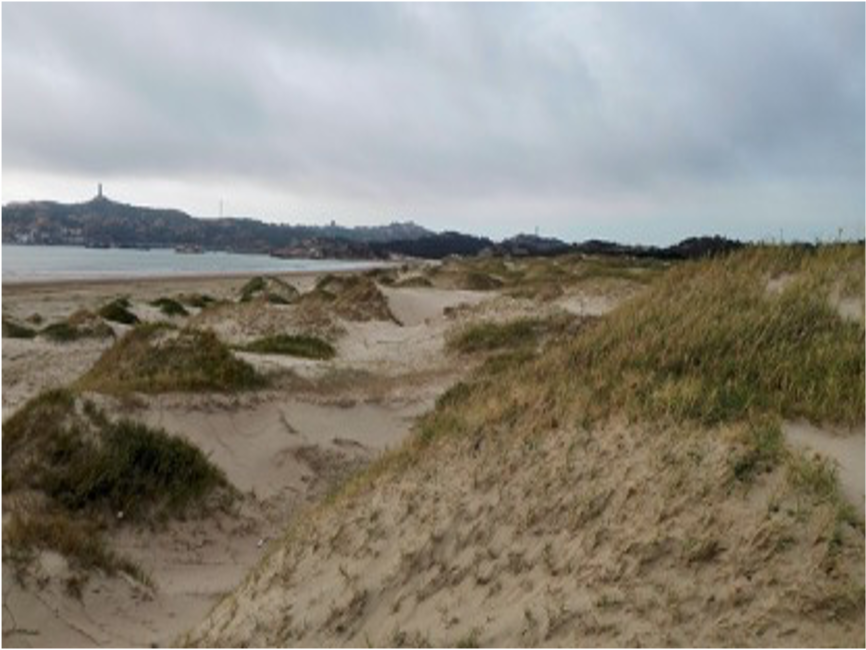
\includegraphics{../figs/sand_buried_plants.png}}}\hspace{5pt}
  \subfloat[\textit{S. littoreus} nebkhas was eradicated and planted with \textit{C. equisetifolia}.]{%
  \resizebox*{6cm}{!}{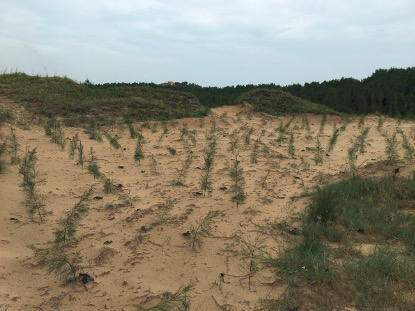
\includegraphics{../figs/damaged_trees.jpg}}}
  \caption{(a) Intensive sand burial on the \textit{Spinifex littoreus} nebkhas on Pingtan Island after typhoon Soudelor (1513) landed in Putian City, Fujian Province, China in August, 2015. (b) The nebkhas formed by \textit{Spinifex littoreus} was stabilized by the planting of an invasive species \textit{Casuarinas equisetifolia} seedlings on Pingtan Island, Fujian Province, China.} 
  \label{fig:sample-pic}
\end{figure}

\label{Introduction-5}
% 我们的研究假设和研究思路
% 我们认为不同的沙埋情形将改变植株的生长方式,是该植物能够适应台风带来的强烈沙埋的关键性因素。
In this study, we assume that the growth of \textit{S. littoreus} can be facilitated with the increase of sand burial, which is probably the key factor for this native plant to adapt to the intense sand burial caused by frequent typhoon events in growing season. Then, the vertical height of ramets, horizontal length of stolons, and biomass allocation of adventitious roots, stems and leaves on stolons of \textit{S. littoreus} under different sand burial levels were simulated and measured in a field experiment, in a growing season on Pingtan Island, Fujian Province, South China.


\section{Material and Methods}
\subsection{Study area}

\begin{figure}
  \centering
  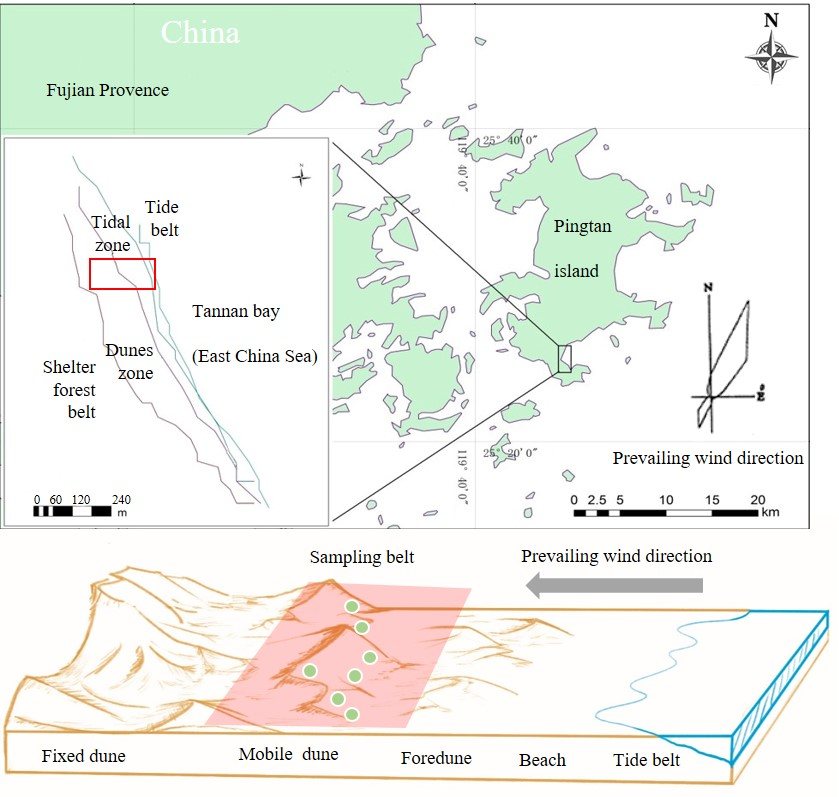
\includegraphics[scale=0.8]{../figs/study_area.jpg}
  \caption{Schematic diagram of the field experiment} 
  \label{fig:map}
\end{figure}

Pingtan Island is located on the eastern coast of Fujian province, South China, with a sub-humid and oceanic monsoon climate. The study area is situated in the southeast of Pingtan Island $(25^{\circ}26'36''-25^{\circ}26'48''N, 119^{\circ}46'09''-119^{\circ}46'21''E)$, and is usually regarded as the most well-preserved coastal sand dunes in China (Figure~\ref{fig:map}) 
\citep{yangDiurnalvariationcharacteristics2017}. 
Annual average temperature is $19.5^{\circ}C$, and precipitation is $1151 mm$. The monsoons are the dominant wind in this area, SE in the summer and NE in the winter, with an annual average wind speed of $6.9 m/s$. A total of 106 typhoons made landfall on Pingtan Island from 1981 to 2019, average 2.65 times per year, and mainly they occurred in July to September. The maximum wind speed can be up to $32.7 m/s$, ultimately leading to the severe sand burial on the psammophytes in this period. Soil is mainly composed of medium to fine sand, with well-sorted grains. Sediments are transported by the wind and intercepted by the ramets and stolons of \textit{S. littoreus}, and a discrete dune mound or hummock is usually formed by aeolian sand deposition within an isolated plant or group of plants \citep{hespCFDFlowDynamics2019}, ultimately developing into a 300 m wide nebkha dominated foredune zone (Figure~\ref{fig:sample-pic}). \textit{S. littoreus} is the dominant species in the study area and the auxiliary plants including \textit{Oenothera drummondii}, \textit{Cynodon dactylon}, \textit{Pluchea pteropoda}, and \textit{Sesuvium portulacastrum} \citep{yangDiurnalvariationcharacteristics2017}. 



\subsection{Methods}
Field experiments were carried out in July, 2016, in Tannan bay, Pingtan Island (Figure~\ref{fig:map}). One study belt without the interruption of animals, pollutants, and apparent human activities was selected in the center of the coastal sand dunes. 
Considering most of the \textit{S. littoreus} were distributed on the windward slope of nebkhas in mobile dunes belt, 35 healthy plants with uniform size were selected for study on this slope (Figure\ref{fig:leeward_swale}). All the observed plants can be well distinguished from surrounding plants, the height of vertical ramets and the length of stolons were all similar with each other before the burial treatments. Stolons of \textit{S. littoreus} on the windward slopes were selected, and labeled with a red cord at points 1/3 and 2/3 of the length from the stolon base to the stolon top. All plant species around the selected plants were manually cleared, and wooden frames $20 cm$ in height (similar to the height of stolons) were set around the selected plants. Later, all the observed plants were fixed with a label, and its serial number was recorded on the label and wooden baffles respectively in order to facilitate the periodic measurements later. The few adventitious roots present on the stolons of the observed plants were completely eliminated, the height of vertical ramets and length of stolons were measured separately before the experiments began. Later, all the plants were buried with sand nearby artificially (Figure~\ref{fig:diagram}, Table~\ref{tab:treatment}), While control groups (CG) were unburied throughout the experiments. 


\begin{figure}
  \centering
  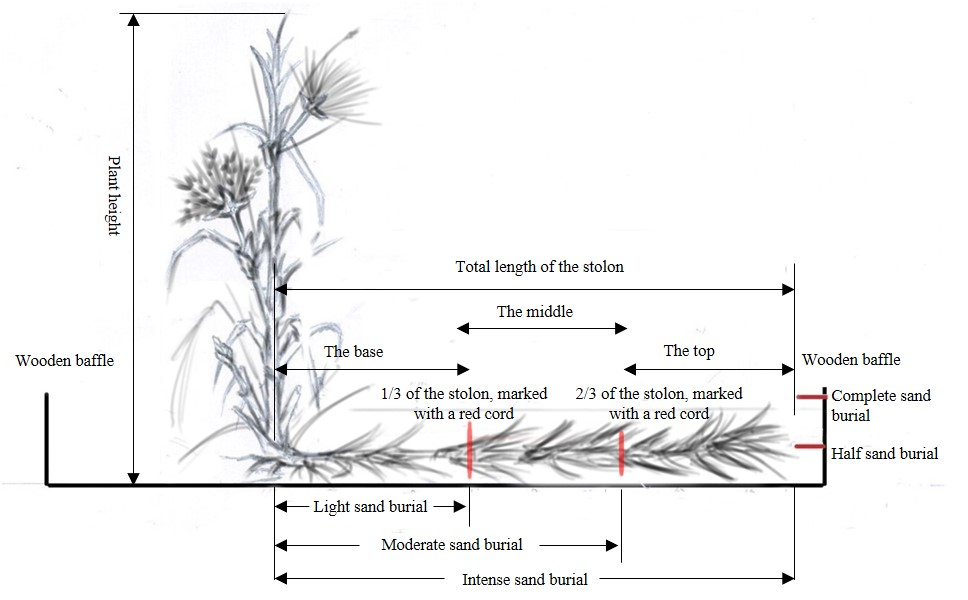
\includegraphics[scale=0.5]{../figs/diagram.jpg}
  \caption{Schematic diagram of the sand burial treatments of the samples} 
  \label{fig:diagram}
\end{figure}

\begin{table}
  \tbl{Sand burial treatments of the plants.}
  {\begin{tabular}{lrrr} 
  \toprule
   Treatment & Burial depth & Burial level \\ 
  \midrule
   CG & No sand burial & No sand burial \\
   HL & Half & Light \\
   HM & Half & Moderate \\
   HI & Half & Intense \\
   CL & Complete & Light \\
   CM & Complete & Moderate \\
   CI & Complete & Intense \\
  \bottomrule
  \end{tabular}}
  \label{tab:treatment}
\end{table}

Since the vertical ramets of \textit{S. littoreus} is relatively high, it is unlikely for them to be completely buried in a single typhoon event (Figure~\ref{fig:sample-pic}a). The treated \textit{S. littoreus}, thus, only the stolons of which were buried at different depths and levels (see Figure~\ref{fig:diagram} and Table~\ref{tab:treatment}). Moreover, some adventitious roots on the stolons of selected plants were observed only a few days after treatments, so the growth parameters of plants were dynamically investigated in 5, 9, 13, 17, 20 days after the sand burial to investigate the response of \textit{S. littoreus} to severe sand burial over a short time scale.

During the measurements, the sand burying the plants was carefully removed to one side in a wooden baffle, and the height of the vertical ramets, the length of the stolons and adventitious roots were all measured with a tape. Considering the uncovering and re-covering of sand will probably affect the gravity signal of plants to sand burial, we finished our measurements in a very short time period (usually 3-5 minutes compared with days of interval) to minimize the potential disturbance, and re-covered the plants to the previous sand burial level with same sand. When the experiments were finished, both above and below ground biomass of plants were collected and separated according to the label on the stolons. Then all the samples were taken back to the laboratory, and the roots, stems and leaves were separated from the stolons, dried in the oven with a temperature of $65^{\circ}C$ for about 24 h until the weight was constant, and then weighed with an analytical balance (accuracy: $0.0001g$).

All the data were calculated with average according to all the replications with standard error as measurement of variability. The results were analysed with Python3 and package Pingouin \citep{vallatPingouinstatisticsPython2018}. For each observed variable, we used repeated measure ANOVA analysis to test if the experimental treatments were verified due to time, and checked the significance $(P<0.05)$.

\section{Results}

\subsection{Influence of sand burial on the growths of \textit{S. littoreus}}

After a 20-day sand burial experiment, we found that the ramet height of \textit{S. littoreus} did not show any significant difference compared with the control group (CG). However, there were significant effects on the growth of horizontal stolons in both half-intense sand burial (HI) and complete-intense sand burial (CI) treatments, particularly the latter (Figure~\ref{fig:lattice}). 
Specifically, the significant effect of sand burial on the stolon growth was firstly observed at 9 days for the CI treatments, while it delayed at 13 days for the HI treatments ($P<0.05$).
Moreover, the growth of horizontal stolons was more enhanced by sand burial in CI treatments than HI treatments, with the stolon length increased by $40.79\%$ in CI treatments, while $24.56\%$ in HI treatments after the end of 20-day sand burial experiment (Figure~\ref{fig:growth} A and B).
Based on that, the proportion of stolon length in top section was increased continuously from $22.09\%$, $25.53\%$ to $46.48\%$, $50.20\%$, for HI and CI treatments, respectively.

\begin{figure}[!h]
  \centering
  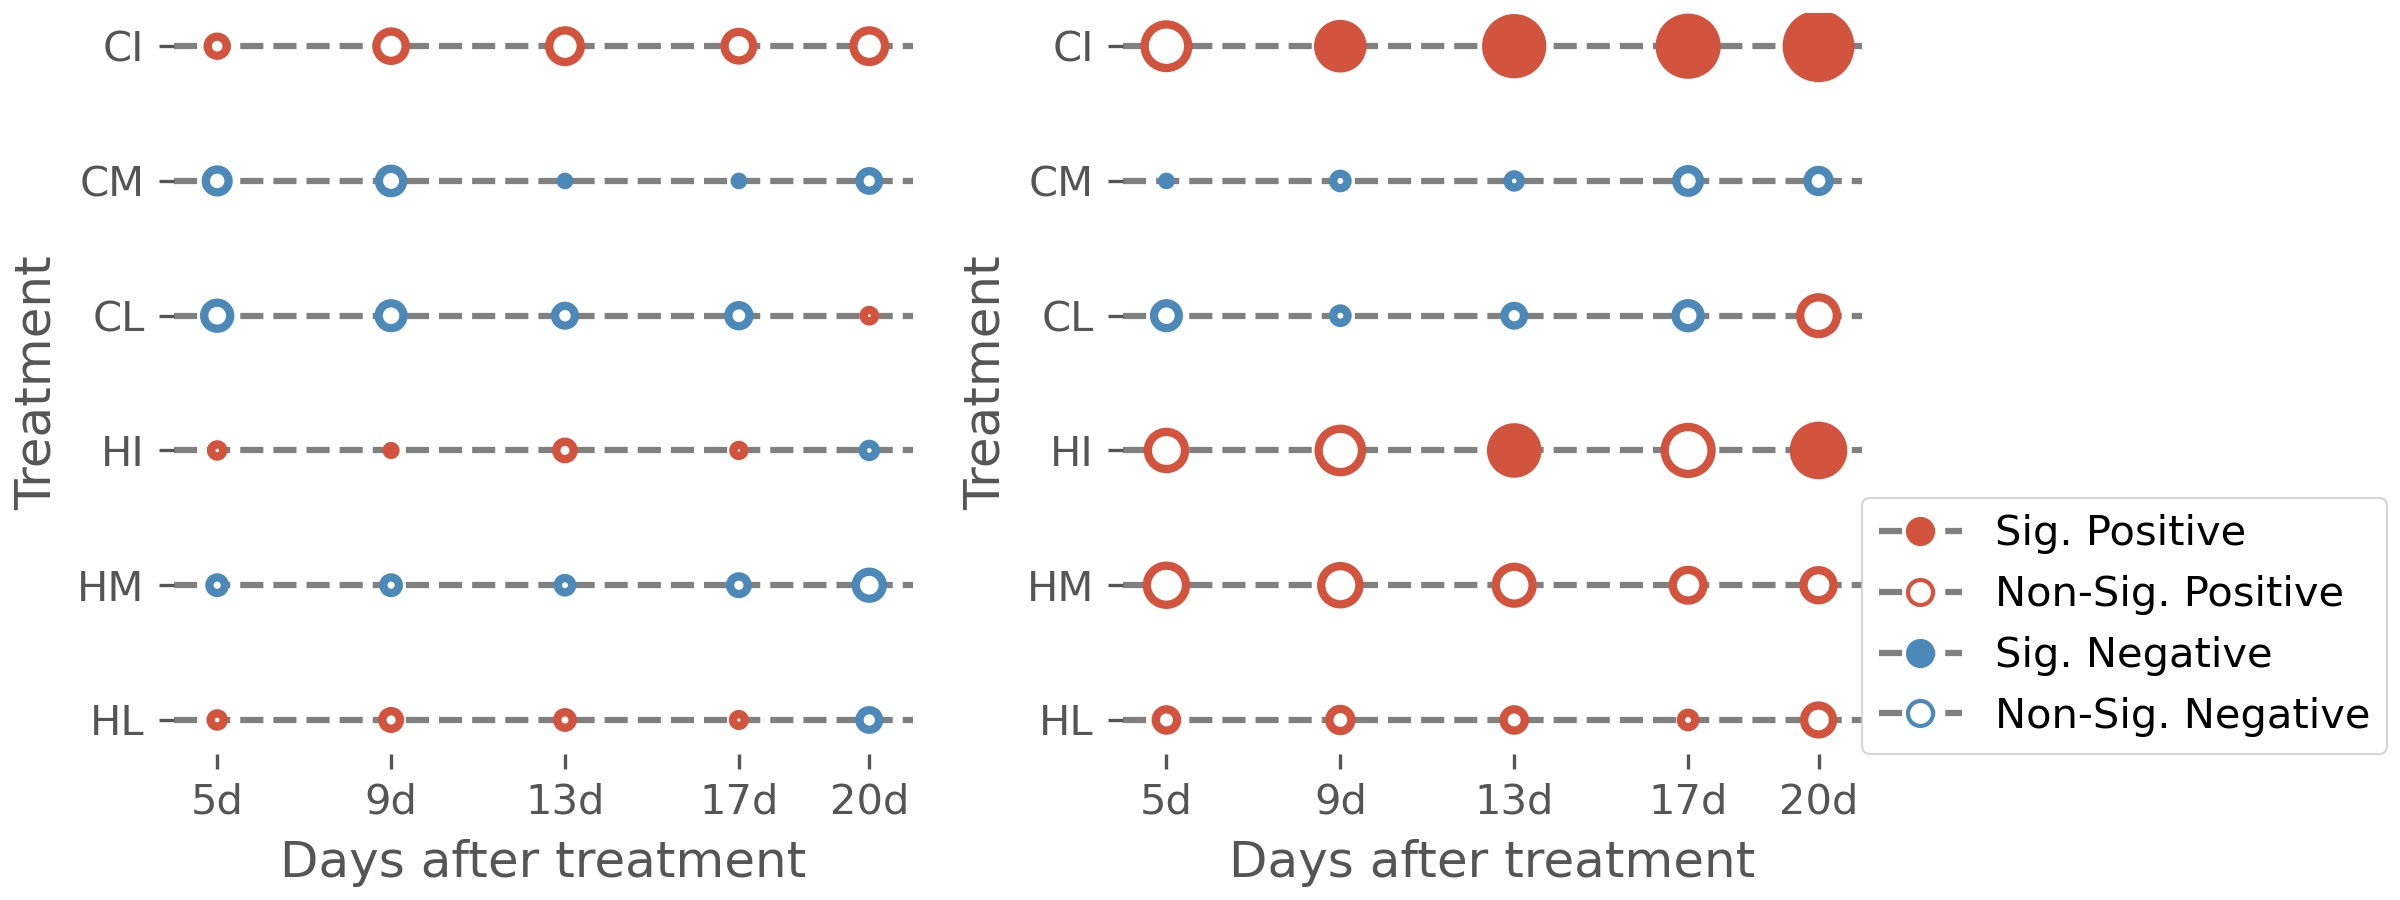
\includegraphics[scale=0.7]{../figs/grid_differences.jpg}
  \caption{
    % 不同沙埋处理下,植株的株高生长(A)与匍匐茎生长(B)同空白对照组之间的差异变化。
    Difference in ramets height growth (\textbf{A}) and horizontal stolons (\textbf{B}) between control group (CG) and different sand burial treatments. The blue dots refer negative (less than CG) while the red dots refer positive (larger than CG) differences. The fulfilled dots are significant different in statistic ($P<0.05$) and size of the dots denotes the size of difference.  
  } 
  \label{fig:lattice}
\end{figure}

\begin{figure}[!h]
  \centering
  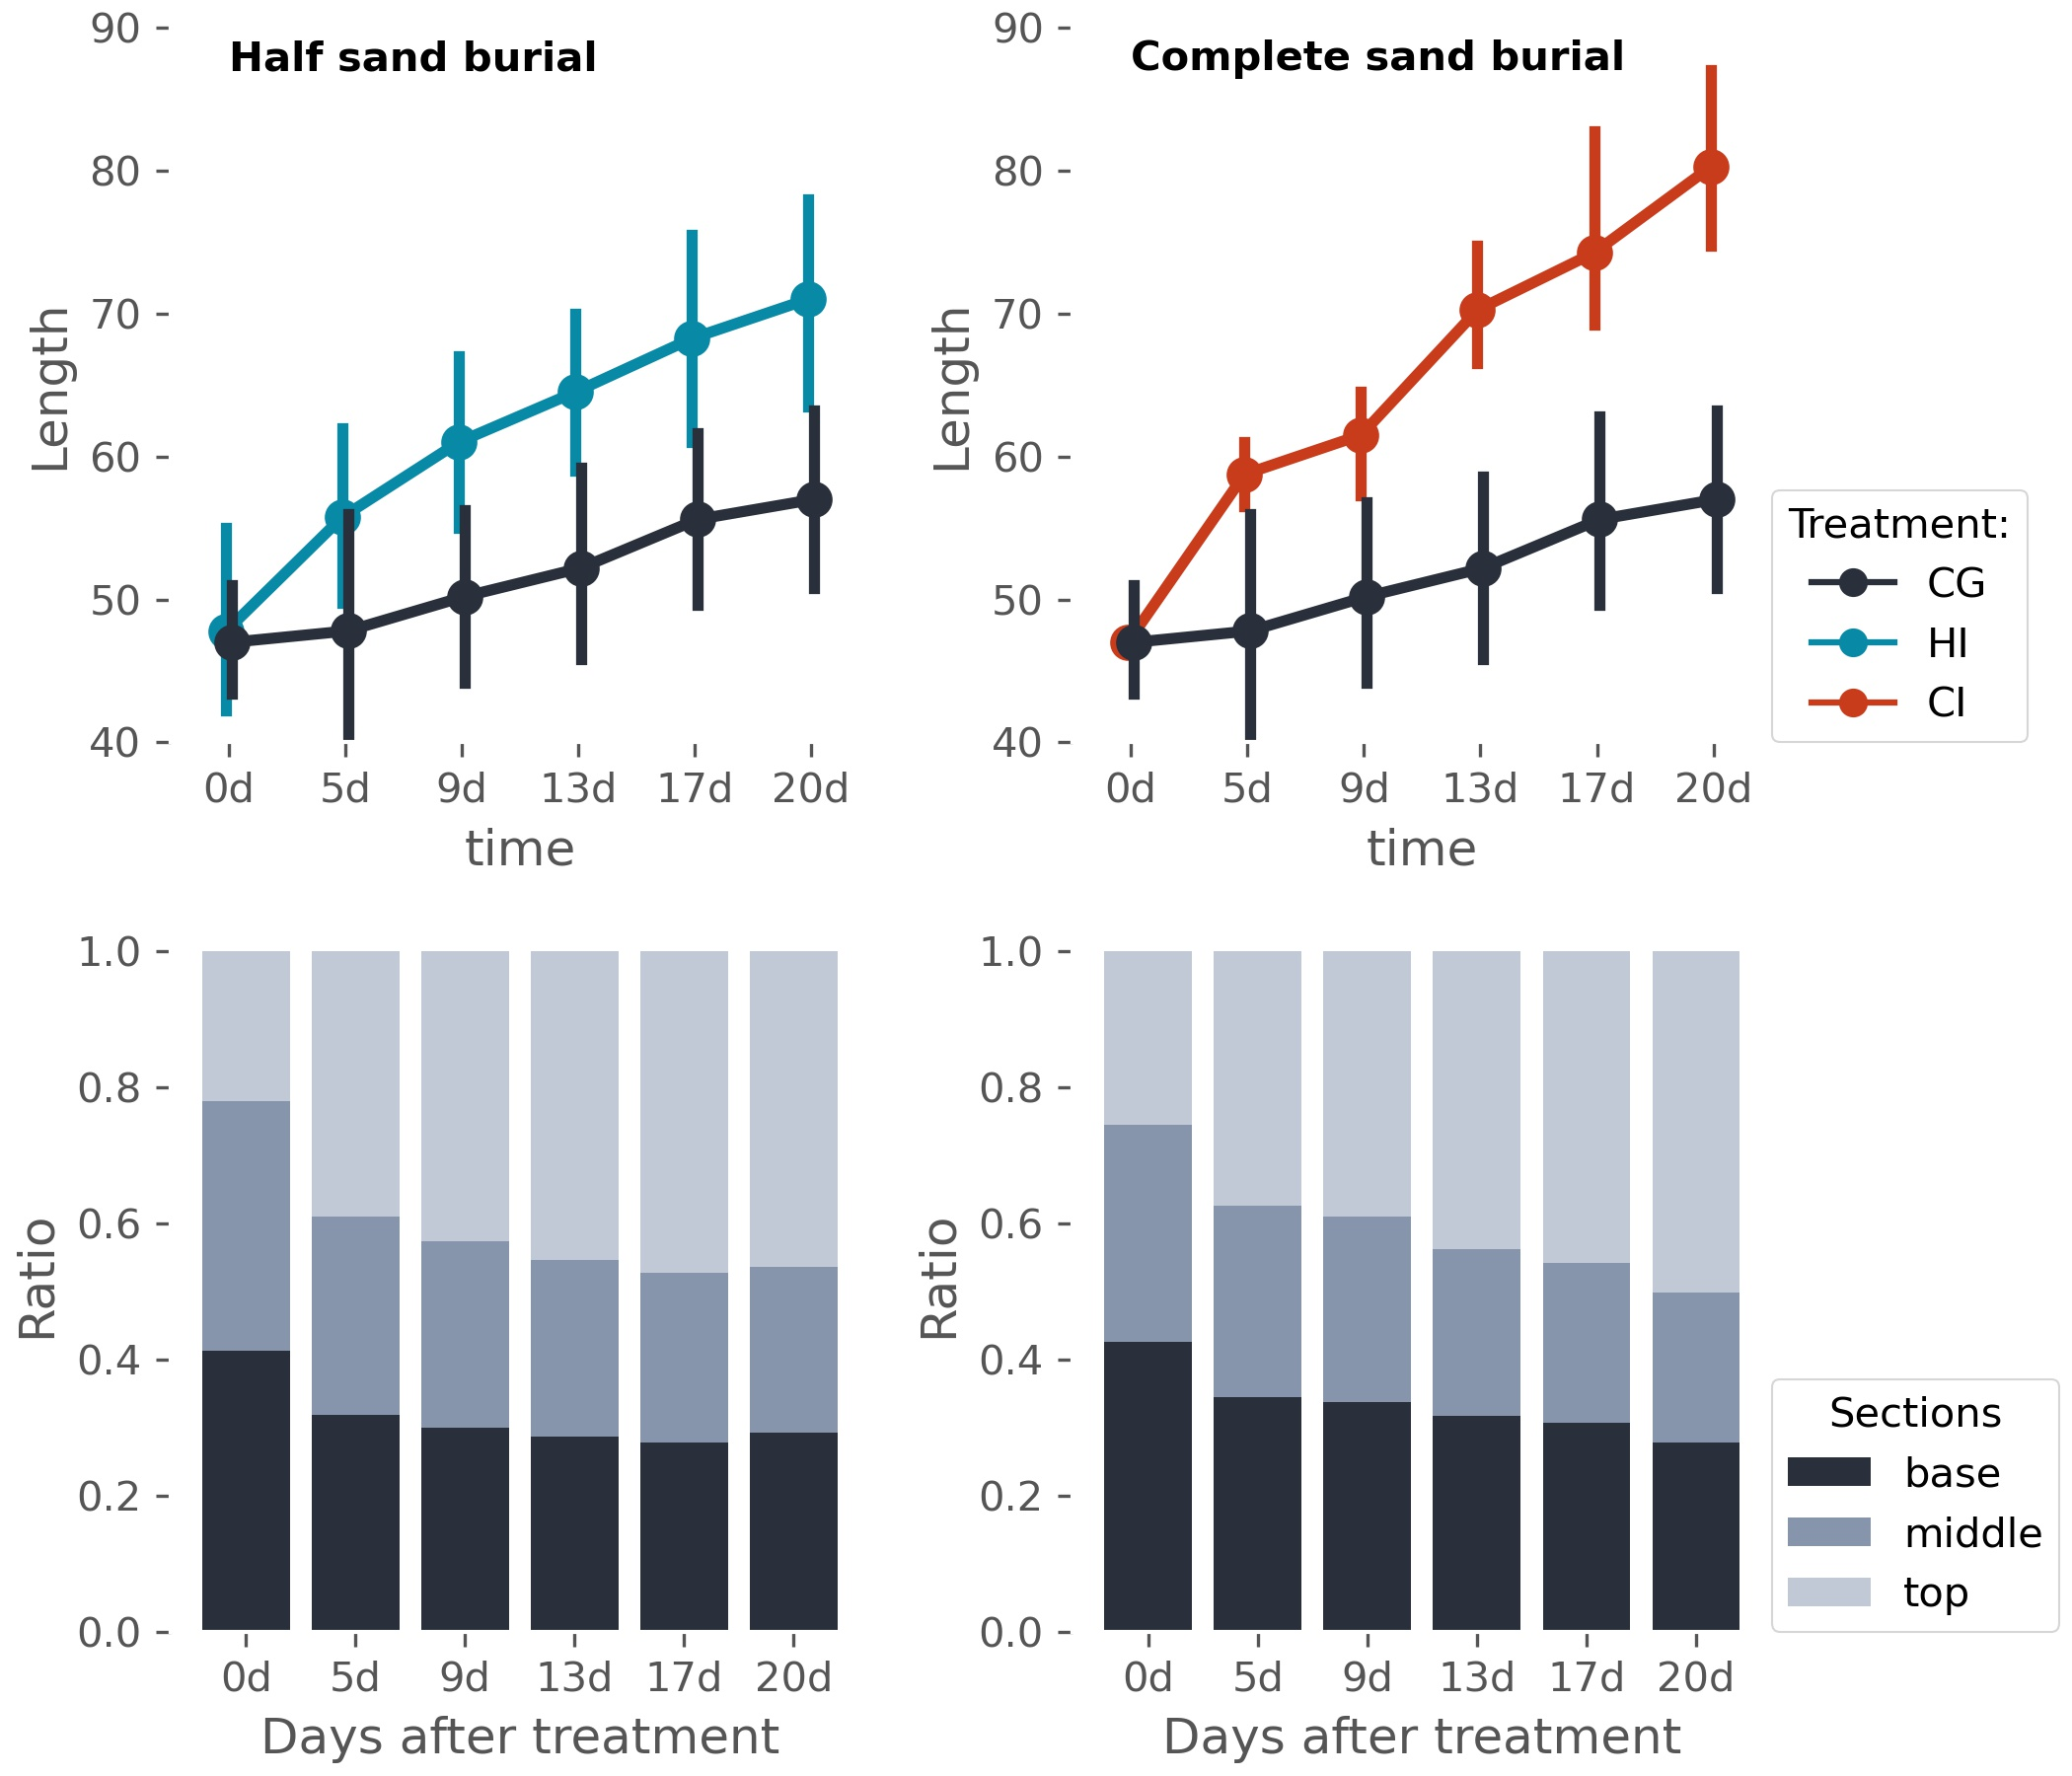
\includegraphics[scale=0.7]{../figs/growth_process.jpg}
  \caption{
    Growth process of horizontal stolons with half-intense (HI) group and complete-intense (CI) group plants.
    \textbf{A} growth of horizontal stolons' length of HI group, compared with the control group (CG).
    \textbf{B} growth of horizontal stolons' length of CI group, compared with the control group (CG).
    \textbf{C} growth of different sections of horizontal stolons' length of HI group.
    \textbf{D} growth of different sections of horizontal stolons' length of CI group.
  }
  \label{fig:growth}
\end{figure}


\subsection{Influence of sand burial on the biomass allocation of \textit{S. littoreus}}
\begin{figure}
  \centering
  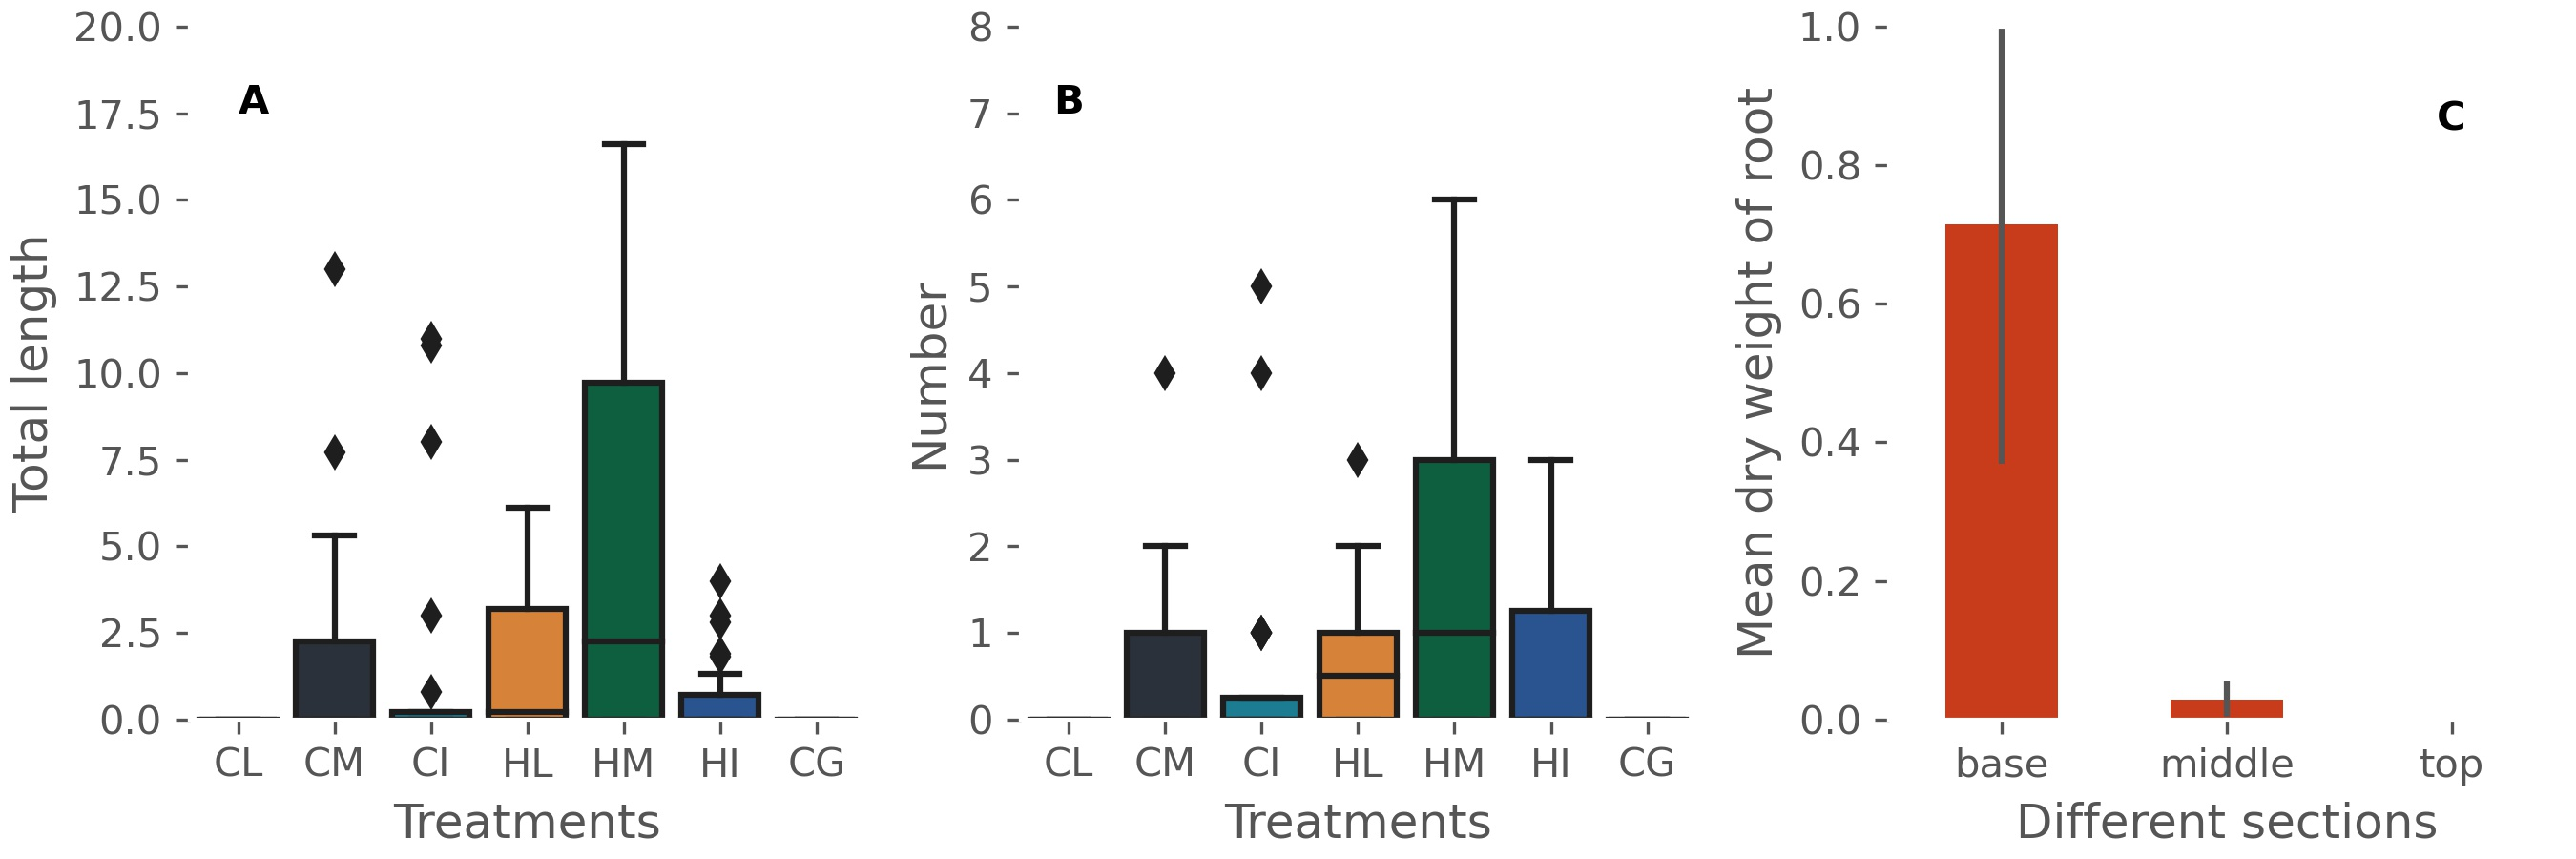
\includegraphics[scale=0.6]{../figs/roots.jpg}
  \caption{
    \textbf{A.} Total length of adventitious roots under different sand burial treatments.
    \textbf{B.} Number of adventitious roots under different sand burial treatments.
    \textbf{C.} Mean dry weights in different sections of horizontal stolons.
  }
  \label{fig:roots}
\end{figure}

\begin{figure}
  \centering
  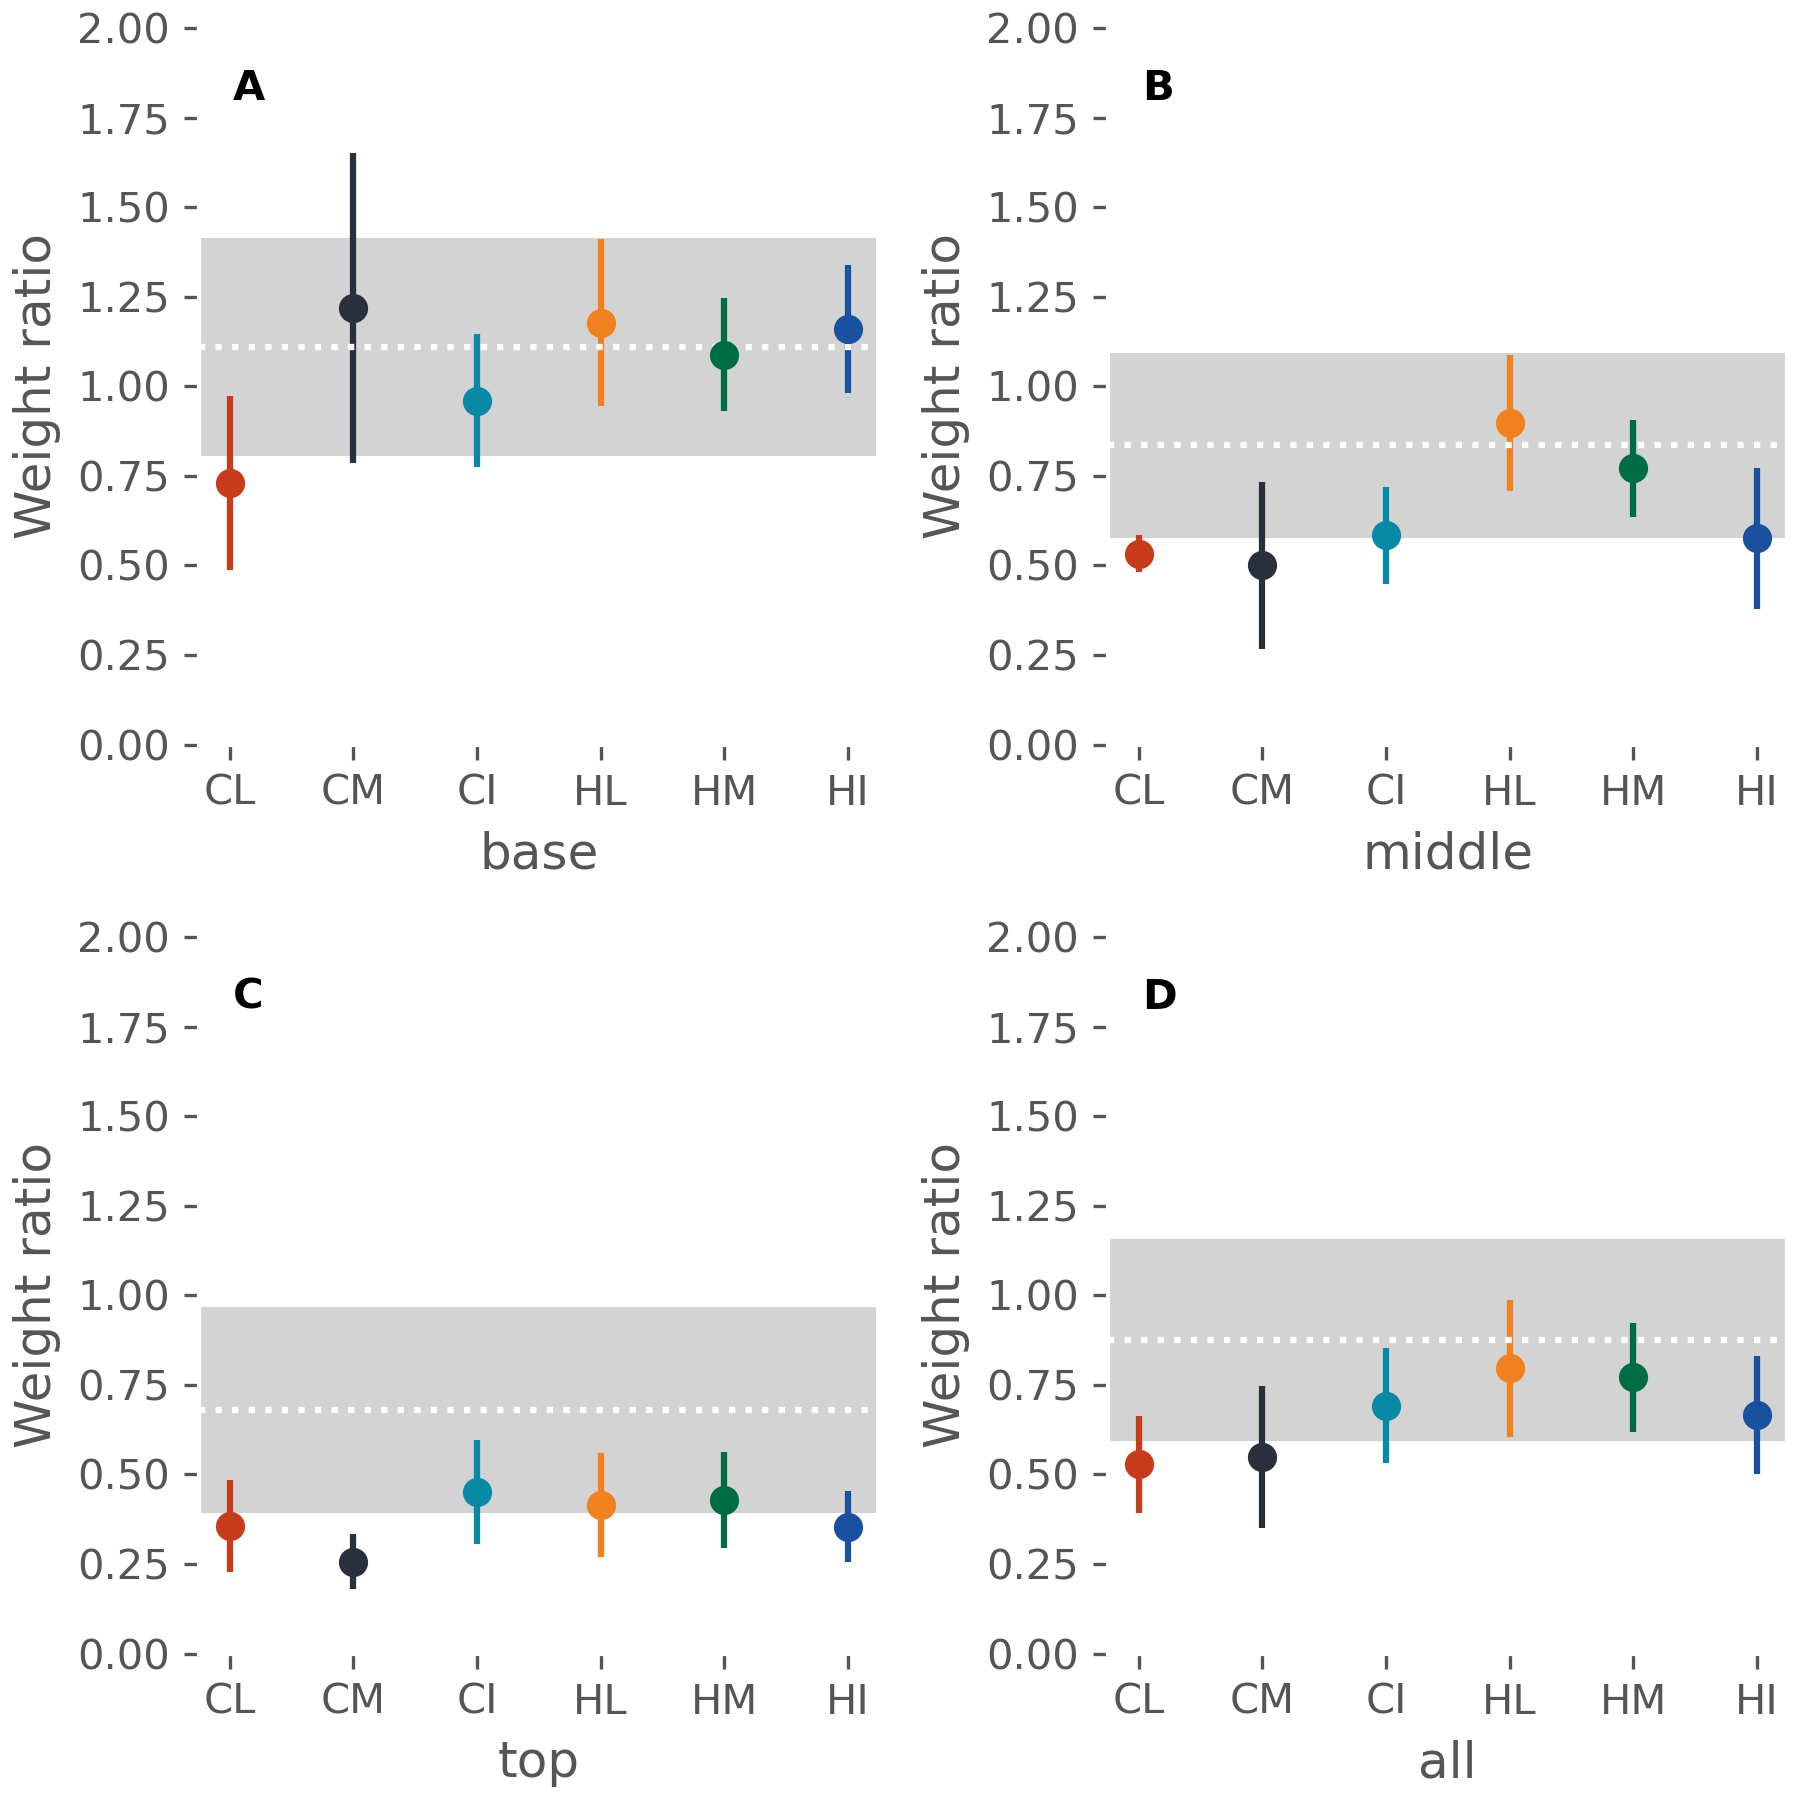
\includegraphics[scale=0.8]{../figs/ratio.jpg}
  \caption{
    Weight ratio between stem and leaf after the end of experiments under different treatments. The white lines denote mean ratio of the control group (CG) while the grey spans denote the standard error of the control group. Weights ratio from different sections were compared one by one (\textbf{A:} base sections, \textbf{B:} middle sections, \textbf{C:} top sections, \textbf{D:} all sections).
  }
  \label{fig:ratio}
\end{figure}

% 大多数的人工沙埋不同程度上促进了不定根的生成,无论是不定根数量还是总长度(Fig3)。
The production of adventitious roots was promoted in most of the sand burial treatments, both in total length and number of roots. The most increase was observed in the HM treatments, and the average root length is $5.1cm$, the average root number is $2$, while no adventitious roots were observed in the CG treatments (Figure~\ref{fig:roots} A and B).
% 而且不定根主要分布在基部,顶端无不定根生成。
The adventitious roots were mainly occurred at the base section of stolons (96\%), and few (4\%) were found at the middle section, while no adventitious roots were found at top sections (Figure~\ref{fig:roots}C).
% 经过20天的沙埋实验,老鼠楽植株茎和叶片的干重比例在不同程度上发生了改变。
The dry weight ratio between stems and leaves of \textit{S. littoreus} was decreased under most of the sand burial treatments compared with the CG treatments, and varied in different sections of stolons. More biomass was allocated to leaves, particularly for the top section of stolons (Figure~\ref{fig:ratio}).

\section{Discussion}

\subsection{Responses of \textit{S. littoreus} to severe sand burial}

Sand burial can reduce the photosynthetic area of species, which finally inhibit the plant performance in coastal sand dunes \citep{hespEcologicalProcessesPlant1991, brownMechanismsSurvivingBurial2018}. Species that withstand sand burial can recover very rapidly by elongating internodes in vertical shoots to overcome this physical barrier \citep{frosiniGlobalChangeResponse2012,keijsersModelingBiogeomorphicEvolution2016, quEffectsSandBurial2017,enriquezAssessingBeachDune2019}. However, this was inconsistent with our study, as we clearly showed that all sand burial treatments on stolons had no significant impact on the vertical growth of its conjoint ramets on the nebkhas. This is probably due to the growth characteristics of \textit{S. littoreus}, which displays both vertical and horizontal extension, the height of its ramets ranges from 40 to 60 cm, and it is virtually impossible to bury the entire vertical ramets by the sand sediments relative to its conjoint stolons during a single typhoon event \citep{yangDiurnalvariationcharacteristics2017}. For the plants on the windward slopes, some unburied leaves are expected to provide photosynthetic substance to sustain the continuous growth of \textit{S. littoreus} even when severe burial occurred (Figure~\ref{fig:sample-pic}). 

Consequently, the rapid growth of ramets height in \textit{S. littoreus} is not considered as the priority for the escape of sand burial, but it inclines to increase the stolon length due to its vulnerability to be buried in a typhoon event, which may contribute to the no significant impact on the ramets height by artificial sand burial in our experiment \citep{maunAdaptationsEnhancingSurvival1994}. Our field investigation further showed that the maximum length of \textit{S.littoreus} stolons could be up to $2-3 m$, which was about to 4-6 times of its ramets height in a frequent sand burial habitat (Figure~\ref{fig:added}b). This is in agreement to the previous study from \citet{woodhouseEffectSpeciesDune1977}, who reported that \textit{Uniola paniculata} tended to grow upward rather than seaward, while \textit{Ammophila breviligulata} preferred to colonize seaward beach surfaces by rhizome growth, which may explain the wider distribution of the latter in an intensive sand burial environment subsequently. 

\begin{figure}[!h]
  \centering
  \subfloat[Developmental period.]{%
  \resizebox*{6cm}{!}{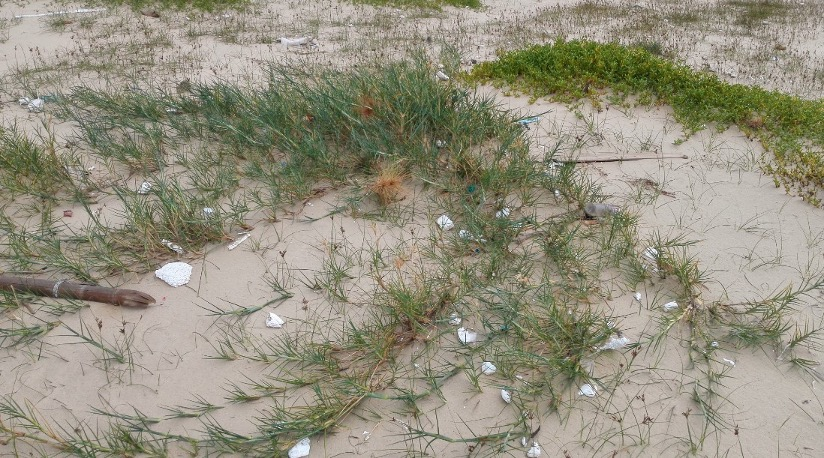
\includegraphics{../figs/fig9b.jpg}}}\hspace{5pt}
  \subfloat[Stabilized period.]{%
  \resizebox*{6cm}{!}{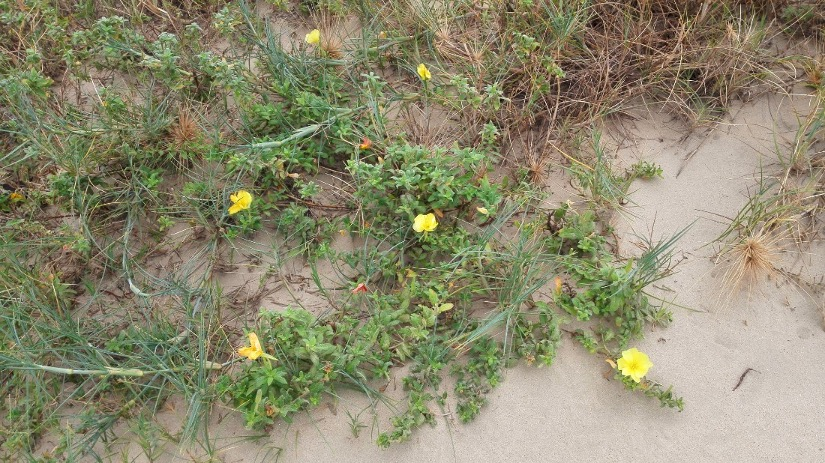
\includegraphics{../figs/fig9a.jpg}}}
  \caption{The stolon length of \textit{S. littoreus} on nebkhas in the developmental period (a) and the stabilized period (b). (Photo was taken in Pingtan Island)} 
  \label{fig:added}
\end{figure}

Extensive colonization of horizontal stolons after sand burial will facilitate the plants to increase its capacity for utilization of water and nutrition, which is especially critical for the establishment of plants in a resource-poor environment, such as coastal sand dunes, and further enhance their growth as the dominant species in coastal sand dunes \citep{divyasreeEcologicalStudyReproduction2019,mendoza-gonzalezBiologicalFloraCoastal2014}. Our results indicated that all sand burial treatments had a significant promotion on the  stolon growth, and complete sand burial had more obvious influence than half sand burial. Species usually stimulate their growing point according to the signal of the gravity signal stresses \citep{zhouAnalysisgrowthstrategy2015}, and increase their node number and internode length to escape this physical barrier \citep{maunEffectsBurialSand1996}. The stresses signal of gravity in complete sand burial was usually stronger than it in half sand burial \citep{wangAdvancesStudiesMorphological2005}. This was consistent with our field investigation, we found that the tall remets of \textit{S. littoreus} could intercept sand sediments, and its conjoint stolons were buried at different levels on nebkhas. The stolon length of \textit{S. littoreus} on nebkhas in developmental period was much longer than it in stabilized period, which can be attributed to the more dynamic sand movement on the fomer (Figure~\ref{fig:added}). 

Production of adventitious roots on the stolons will enhance the capacity of plants to use limited soil water and nutrition, and change the biomass and growth rhythms of plants \citep{martinezResponsesDuneMosses1999,dechAdventitiousRootProduction2006}. Our results indicated that the adventitious roots were produced on the \textit{S. littoreus} stolons in most of the sand burial treatments, both total length and number of roots were increased compared with the CG treatments, which will facilitate their revitalization from sand burial caused by typhoon events. More adventitious roots were allocated to the stolon base after sand burial. Generally, sand burial depth is deeper on the stolon base than other stolon sections due to more sand sediments accumulated around the conjoint ramets, which will increase the capacity for root growth and can improve their access to soil water and nutrition \citep{yuanEffectsSandAccretion1993}. Moreover, \textit{S.littoreus} has a fibrous root system, and adventitious roots are initially produced from the primordium in the stolon node. However, only the primordium in the stolon base can develop well and finally break through the cuticular layer to produce the adventitious roots \citep{hochholdingerWeedsCropsGenetic2004}. 

The top section of stolon is usually the least buried sections of stolons, as the photosynthetic organ, more leaves emerging on the top of stolon will reduce the risk of plants from further sand burial, increase their light capture for photosynthesis and carbon gain \citep{yuanEffectsSandAccretion1993, shiEffectsSandBurial2004, brownMechanismsSurvivingBurial2018}, and ensure enough supply of carbohydrates for plants to escape the sand burial. Our study further supported this conclusion, and we found that a larger percent of leaves were observed on the top of stolon compared with other stolon sections. \citet{gilbertGrowthResponsesCoastal2008} also demonstrated that sand burial could increase the leaf area in mobile dune species, which fully or partially replaced the lost photosynthetic leaf area, so the shoot must elongate its stem to keep newly produced leaves above the sand surface subsequent to the sand burial. Consequently, in order to reduce the cost of stem tissue production, the stem tissue density of species is usually negative to the maximal stem elongation rate \citep{frosiniGlobalChangeResponse2012}. We also found that the extension rate was faster in top of stolon than other stolon sections of \textit{S.littoreus}, and it grew even faster as the sand burial prolonged. Consequently, the dry biomass ratio of stem to leaves showed a decreasing trend from the stolon base to the stolon top of \textit{S. littoreus} in all sand burial treatments. 


\subsection{Significance of \textit{\textit{S. littoreus}'} adaptation to sand burial}

% 凭借上述机制,我们的结果表明老鼠楽能够有效在近地表被严重的沙埋情况下加速生长并存活下来。在热带和亚热带地区的海岸,频繁的台风常常为迎风坡带来数十厘米厚的沙埋,尽管这样的沙埋足以阻止大多数植物在此生长,但老鼠楽凭借其独特的适应能力在此占据来绝对优势。
Response of plants to sand burial is usually species specific, and the growth of plants will be enhanced under optimal sand burial rate \citep{noletUAVimagingModelGrowth2018}. We found that \textit{S.littoreus} can adapt to the severe sand burial caused by frequent typhoons in our study area, and will revitalize later by increasing the horizontal stolon length, producing abundant adventitious roots on the stolon base and allocating more biomass to leaves on the stolon apex \citep{yuanEffectsSandAccretion1993}. However, if the sand burial rate is over some threshold, the growth of sand dune species will be inhibited \citep{maunEffectsBurialSand1996, shiEffectsSandBurial2004}. Our field investigation showed that few \textit{S. littoreus} can be found on the leeward slope of nebkhas (Figure~\ref{fig:leeward_swale}a), which can be attributed to the excessive sand burial on both ramets and conjoint stolons of \textit{S. littoreus}. Absence of photosynthesis area, combined with the continuous depletion of reserves previously stored in the plants \citep{frosiniGlobalChangeResponse2012}, finally lead to the failure of \textit{S. littoreus} escaped from excessive sand burial on leeward slope of nebkhas (Figure~\ref{fig:leeward_swale}a).  Similarly, if the sand burial rate is below some threshold, the species that can not withstand the severe sand burial will co-occur with those resistant to it. We found that low to moderate sand burial treatments had no significant impact on the stolon extension of \textit{S.littoreus}, which will not favor its access to the more habitats for soil water and nutrition, and further weaken its advantages as the dominant species with the decrease of sand burial rate. This is also consistent with our field investigation, \textit{Oenothera drummondii}, an invasive species widely distributed on the stabilized dune in South China, is more frequently co-occurred with \textit{S.littoreus} on the nebkhas stabilized by \textit{C. equisetifolia} in our study area (Figure~\ref{fig:added}a and Figure~\ref{fig:leeward_swale}b).

We consider that the capacity of \textit{S. littoreus} stabilizing and building the coastal sand dunes along the coastline of South China has been  underestimated or neglected by the local government, and the coastal managers should allow the regular input of wind-blown sand towards this unique species for the protection and building of coastal sand dunes \citep{noletUAVimagingModelGrowth2018}, which can greatly mitigate the loss from coastal hazards in this region. So the nebkhas formed by \textit{S. littoreus} should be kept dynamic rather than stabilized by some invasive species such as \textit{C. equisetifolia} in Southeast China. Otherwise, it will further increase the risk of species invasion on coastal sand dunes, such as \textit{O. drummondii}. Consequently, this native and highly adaptive species will gradually be replaced and eradicated, and  the degradation of coastal dune systems in this region was also expected to be aggravated.

\begin{figure}
  \centering
  \subfloat[Leeward.]{%
  \resizebox*{6cm}{!}{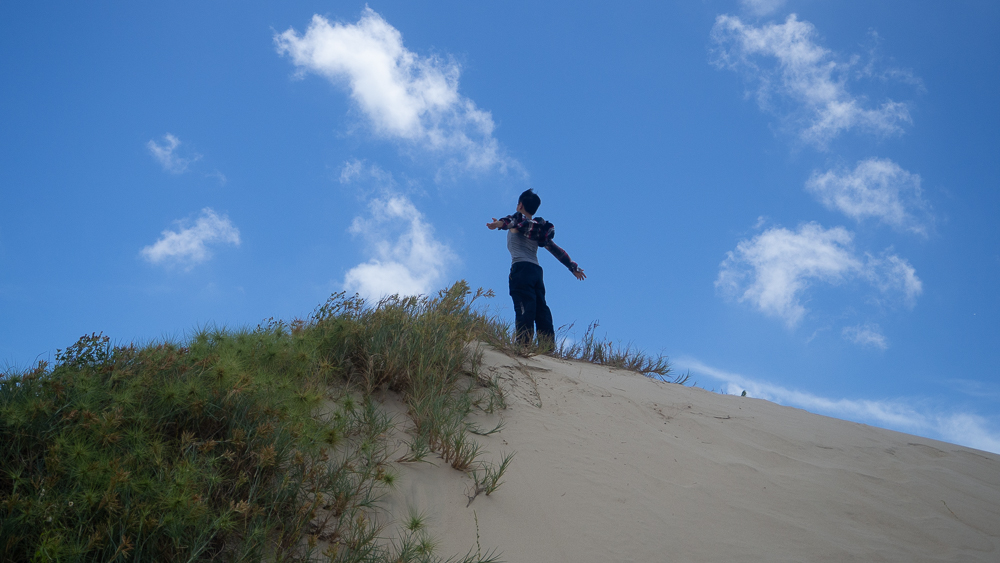
\includegraphics{../figs/leeward.jpg}}}\hspace{5pt}
  \subfloat[Swale.]{%
  \resizebox*{6cm}{!}{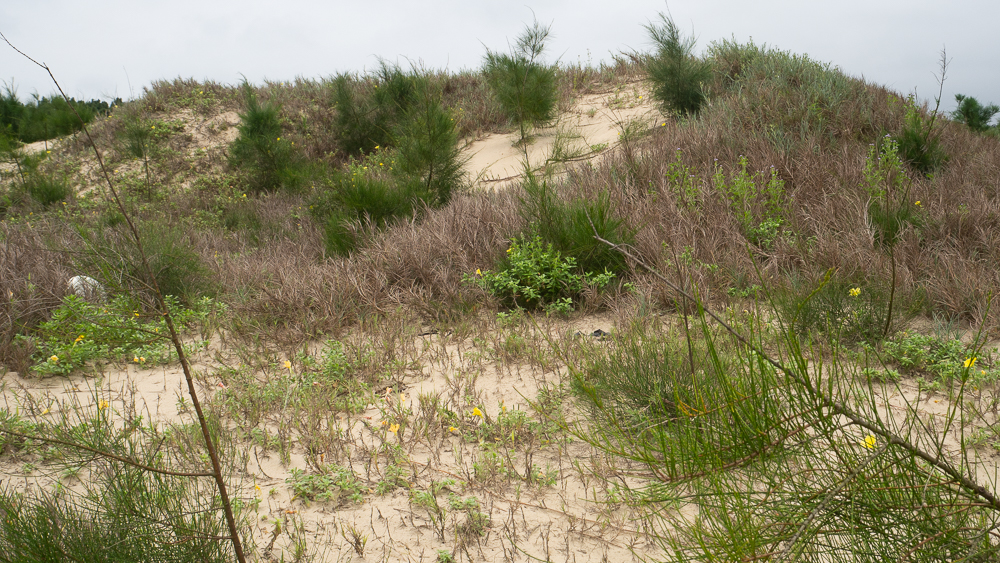
\includegraphics{../figs/swale.jpg}}}
  \caption{(a) Leeward is the most severe sand-burial position where few plants can survive there, including \textit{S. littoreus}. (b) Swales are much better habitats for plants because of little sand burial. However, \textit{S. littoreus} can not be dominant in this area because of heavy competition. Photo was taken in Pingtan Island.} 
  \label{fig:leeward_swale}
\end{figure}

\section{Conclusion}
The following conclusions may be made:

(1) All sand burial treatments had no significant impact on the 
ramets height of \textit{S. littoreus}. However, compared with the CG treatments, they significantly enhanced the stolon extension of \textit{S. littoreus} under intense sand burial (HI and CI) treatments by 24.56\% and 40.79\%, respectively.

(2) Sand burial stimulated the production of adventitious roots mainly on stolon base, and enhanced the germination of leaves on the stolon top of \textit{S. littoreus}.

(3) \textit{S. littoreus} can adapt to the severe sand burial in growing season, it can be considered as one of the optimal species for stabilizing and building the coastal sand dunes in South China. 


\section*{Acknowledgement(s)}

% An unnumbered section, e.g.\ \verb"\section*{Acknowledgements}", may be used for thanks, etc.\ if required and included \emph{in the non-anonymous version} before any Notes or References.
Thanks to Patrick Hesp for his assistance with editing our paper. Thanks to Zhiqiang Ye for his assistance with the field experiment.

\section*{Disclosure statement}

% An unnumbered section, e.g.\ \verb"\section*{Disclosure statement}", may be used to declare any potential conflict of interest and included \emph{in the non-anonymous version} before any Notes or References, after any Acknowledgements and before any Funding information.
The authors declare no competing interests. 

\section*{Funding}

% An unnumbered section, e.g.\ \verb"\section*{Funding}", may be used for grant details, etc.\ if required and included \emph{in the non-anonymous version} before any Notes or References.
This research was supported by National Science Foundation (Grant No. 41101011; 41801101). 


% \section*{Notes on contributor(s)}

% An unnumbered section, e.g.\ \verb"\section*{Notes on contributors}", may be included \emph{in the non-anonymous version} if required. A photograph may be added if requested.


% \section*{Nomenclature/Notation}

% An unnumbered section, e.g.\ \verb"\section*{Nomenclature}" (or \verb"\section*{Notation}"), may be included if required, before any Notes or References.


% \section*{Notes}

% An unnumbered `Notes' section may be included before the References (if using the \verb"endnotes" package, use the command \verb"\theendnotes" where the notes are to appear, instead of creating a \verb"\section*").

\bibliographystyle{tfcse}
\bibliography{Pingtan_ecology}

\end{document}
